\subsection{Efectos en la se\~nal y el espectro}

\subsection{Buenos par\'ametros para se\~nales espec\'ificas}

\subsubsection{Sonidos}

!!!!!!!!!!!!!!!!!!!!!!!!!!1

\subsubsection{Im\'agenes}

Aqu\'i presentamos un gr\'afico que muestra la relaci\'on entre
ruido introducido y mejora del PSNR.
Es importante notar que cada uno de estos resultados fue el trabajo
de una optimizaci\'on manual\footnote{Ver el ap\'endice de tablas
para los resultados num\'ericos y los par\'ametros utilizados},
y que si bien pensamos que puede
ser automatizada, no nos result\'o evidente la manera de hacerlo.
Dado que deben optimizarse dos par\'ametros simultaneamente y
las funciones a optimizar parecen registrar varios m\'inimos
locales.

Las im\'genes usadas fueron \texttt{Red\_cuadrada.pgm} y
\texttt{masterVoice\_cuadrada.pgm}.
Dado que la primera es de un tama\~no peque\~no utilizamos
unicamente los filtros est\'andar. Para la segunda utilizamos
tambi\'en los algoritmos por bloques.

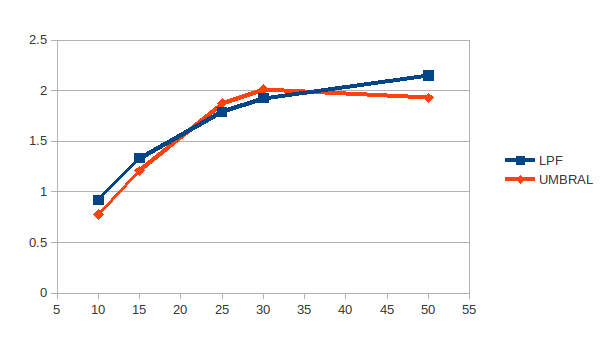
\includegraphics[width=14cm]{red_psnr.png}

{\center \textsc{Decibeles ganados - porcentaje de ruido introducido}\\
	Im\'agen \texttt{Red\_cuadrada.png} }


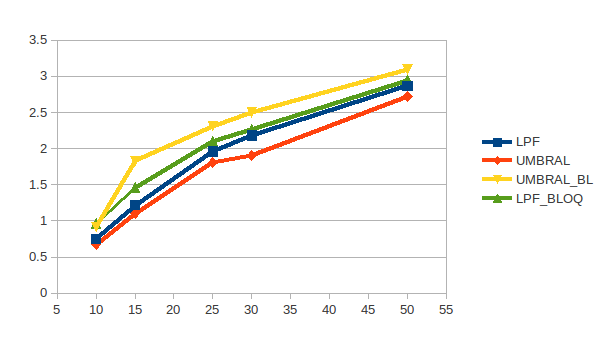
\includegraphics[width=14cm]{voice_psnr.png}
{ \center \textsc{Decibeles ganados - porcentaje de ruido introducido}\\
  \center Im\'agen \texttt{masterVoice\_cuadrada.png} }

\subsection{Tiempo de corrida}

La diferencia, en tiempo, entre trabajar con el espectro de toda la
im\'agen y filtrar de a bloques se ve en esta im\'agen:

AKSJDAKJSDNASKJN

Aqu\'i se comparan los tiempos de ejecuci\'on de un filtro por bloques
para distintos tama\~nos de bloque\footnote{En ambos casos no se hace
distinci\'on entre los filtros de umbral o
pasa-bajos, ya que esto no es relevante para la toma de tiempos.}:

JANSDKAJNDKAJNDKASJDN


